% Created 2024-10-21 Mon 01:31
% Intended LaTeX compiler: pdflatex
\documentclass[11pt]{article}
\usepackage[utf8]{inputenc}
\usepackage[T1]{fontenc}
\usepackage{graphicx}
\usepackage{longtable}
\usepackage{wrapfig}
\usepackage{rotating}
\usepackage[normalem]{ulem}
\usepackage{amsmath}
\usepackage{amssymb}
\usepackage{capt-of}
\usepackage{hyperref}
\usepackage{enumitem}
\usepackage{breqn}
\author{Charles Gannon}
\date{\today}
\title{Astro 204}
\hypersetup{
 pdfauthor={Charles Gannon},
 pdftitle={Astro 204},
 pdfkeywords={},
 pdfsubject={},
 pdfcreator={Emacs 29.4 (Org mode 9.8)}, 
 pdflang={English}}
\begin{document}

\maketitle
\tableofcontents

\section{Streamlines}
\label{sec:org7364290}



\begin{enumerate}[label=\alph*)]

   \item
       The streamline in spherical coordinates are determined by the equation
       \begin{equation}
          \frac{dr}{v_{r}} = r \frac{d \theta}{v_{\theta}} = \frac{dz}{v_z}.
       \end{equation}
       For the case $v_r = a$, $v_{\theta} = b$, $v_{z} = 0$, the equation of the stream lines becomes
       \begin{equation}
          \frac{d r}{d \theta} = r \frac{a}{b},
       \end{equation}
       a first order differential equation.
       The equation has the solution
       \begin{equation}
          r(\theta) = C e^{(a / b) \theta},
       \end{equation}
       where C is a constant of integration.
       This is the form of a logarithmic spiral, which is plotted in fig. \ref{fig:spiral}.
   \item
      For the case $v_r = ar^{2}$, $v_{\theta} = br^{2}$, $v_{z} = 0$, the equation of the stream lines remains the same
      \begin{equation}
         \frac{d r}{d \theta} = r \frac{a}{b},
      \end{equation}
      which is identical to case (a).

   \item
      The change in mass, $\dot{M}$ along a circular shell is
      \begin{equation}
         \dot{M} = 2 \pi r \Sigma v_{r}
      \end{equation}

      Rearranging gives
      \begin{equation}
         \Sigma = \dot{M} / (2 \pi r v_{r}),
      \end{equation}
      which becomes $\Sigma(r) = \dot{M} / (2 \pi b r)$ for part (a) and $\Sigma = \dot(M) / (2 \pi b r^{3})$ for part (b).
\end{enumerate}

\begin{figure}[htbp]
\centering
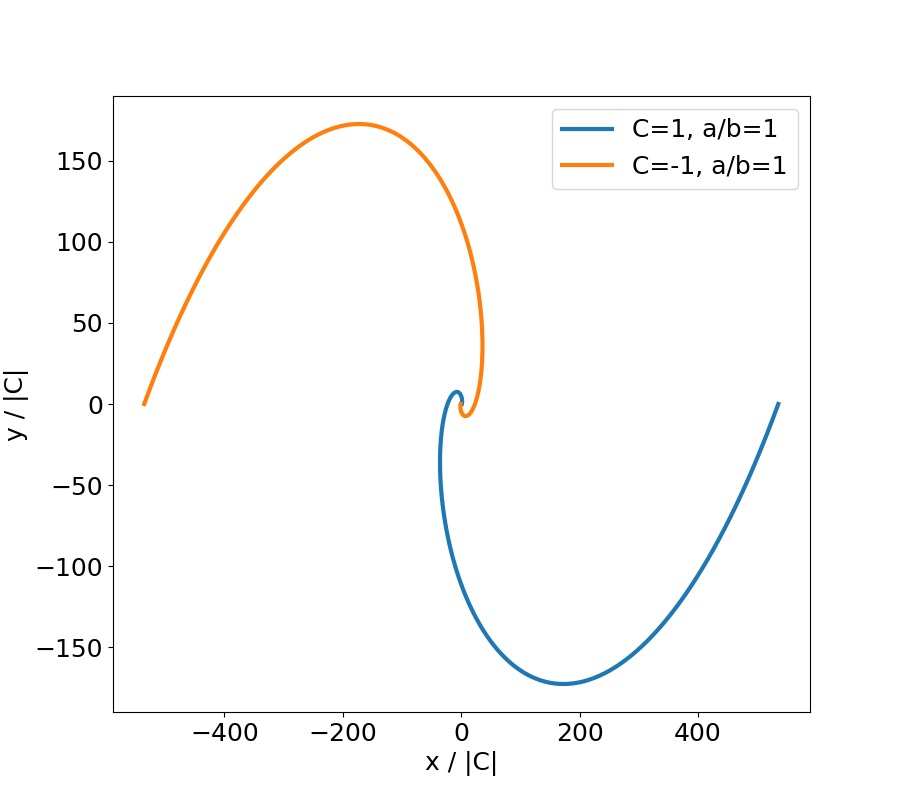
\includegraphics[width=.9\linewidth]{../plots/spiral.png}
\caption{\label{fig:spiral}The streamlines for part (a) and part (b)}
\end{figure}
\section{The Energy Equation}
\label{sec:orge84c28e}
Since the no work is being done on the system by external forces \(F \cdot \vec{v} = 0\), which can be stated as
\begin{equation}
   \frac{\partial E}{\partial t} + \vec{\nabla} \cdot (F_E \vec{v}) = 0
\end{equation}
where \(F_E = E + P\) and E = \(\frac{1}{2} \rho v^2 + \rho \epsilon\).
Plugging in yields
\begin{dmath}
   0 = \frac{1}{2} v^{2} \frac{\partial \rho}{\partial t} + \rho \vec{v} \cdot \frac{\partial \vec{v}}{\partial t} + \rho \frac{\partial \epsilon}{\partial t} + \epsilon \frac{\partial \rho}{\partial t} + \frac{1}{2} \rho v^{2} \vec{\nabla} \cdot \vec{v} + \vec{v}\cdot\vec{\nabla} (\frac{1}{2} \rho v^{2}) + \rho \epsilon \vec{\nabla} \cdot \vec{v} + \vec{v} \cdot \vec{\nabla} (\rho \epsilon) + P \vec{\nabla} \cdot \vec{v} + \vec{v} \cdot \vec{\nabla} P.
\end{dmath}
Grouping like terms and doing algebra gives
\begin{dmath}
   \left( \rho \frac{\partial \epsilon}{\partial t} + \rho \vec{v} \cdot \vec{\nabla} \epsilon + P\vec{\nabla} \cdot \vec{v} \right)
  + \epsilon \left(\vec{v} \cdot \vec{\nabla} \rho + \frac{\partial \rho}{\partial t} + \rho \vec{\nabla} \cdot \vec{v} \right)
  + \frac{1}{2} v^2 \left(\frac{\partial \rho}{\partial t} + \rho \vec{\nabla} \cdot \vec{v} + \vec{v} \cdot \vec{\nabla} \rho \right)
  + \vec{v} \cdot \left(\vec{\nabla} P + \frac{\partial \vec{v}}{\partial t} + \rho \left(\vec{v} \cdot \vec{\nabla} \right) \vec{v} \right),
\end{dmath}
which can be further simplified by realizing the \(\epsilon\) and \(\frac{1}{2} v^2\) term is 0 by continuity (\(\frac{\partial \rho}{\partial t} + \vec{\nabla} \cdot (\rho \vec{v}) = 0\))and the \(\vec{v}\) term is 0 by momentum conservation.
   Therefore,
\begin{equation}\label{eq:lemma}
   \rho \frac{\partial \epsilon}{\partial t} + \rho \vec{v} \cdot \vec{\nabla} \epsilon + P\vec{\nabla} \cdot \vec{v} = 0
\end{equation}
The fundamental equation of thermodynamics is \(d\epsilon = T ds + \frac{P}{\rho^{2}} d \rho\), which can be rewritten as
\begin{equation}\label{eq:thermofund}
   \rho T \frac{ds}{dt} = \rho \frac{d \epsilon}{d t} - \frac{P}{\rho} \frac{d \rho}{dt}
\end{equation}
Using the chain rule on \(\frac{d \epsilon}{dt}\) gives
\begin{equation}
   \frac{d \epsilon}{dt} = \frac{\partial \epsilon}{\partial t} + \vec{v} \cdot \vec{\nabla} \epsilon,
\end{equation}
likewise using the chain rule for \(\frac{d \rho}{d t}\) and plugging in the continuity equation gives
\begin{equation}
   \frac{d \rho}{dt} = \frac{\partial \rho}{\partial t} + \vec{v} \cdot \vec{\nabla} \rho  = - \rho \vec{\nabla} \cdot \vec{v}.
\end{equation}
Plugging into eq. \ref{eq:thermofund} gives
\begin{equation}
    \rho T \frac{ds}{dt} = \rho \frac{\partial \epsilon}{\partial t} + \rho \vec{v} \cdot \vec{\nabla} \epsilon + P \vec{\nabla} \cdot \vec{v}
\end{equation}
Which when plugged into eq. \ref{eq:lemma} gives
\begin{equation}
   \frac{ds}{dt} = 0
\end{equation}
\section{Entropy}
\label{sec:org98d708c}
\begin{enumerate}[label=\alph*)]
   \item
       Starting from the statistical mechanics definition of entropy $\sigma = \log g$, where g is the number of available of states and given the distribution of particles per unit volume in 6D phase space $f(\vec{x}, \vec{v}, t)$ we can understand the provided equation (4).
       Assuming each constant volume element in phase space can hold an equal number of states, the amount of volume occupied by a particle is equal to the number of equivalent states for that particle.
      Therefore, the number of states per particle can be thought of as $f^{-1}$ and the entropy per particle becomes $\sigma = - \log f$.
      The total entropy of the system per unit volume at a point in space and time can be calculated by averaging over all velocity states, and weighting by the number of particles per state.
      Calculating the thermodyamic entropy $S = k \sigma$, and writing the weighted statistical average explicitly gives
      \begin{equation}\label{eq:spv}
         s = -k \int_{\text{all} \vec{v}} f \ln f d^3 v ,
      \end{equation}
      where s is the entropy per unit volume of the system.
   \item
      For a maxwellian, $f(\vec{x}, \vec{v}, t) = n f_{\text{Max}}(\vec{v})$ plugging into equation eq. \ref{eq:spv} gives
      \begin{equation}
         S = -4 k a^3 \pi^{-3/2} n \int_{\mathbb{R}} v^{2} e^{-(av)^{2}} \ln \left[ n \left(\frac{a^{2}}{\pi}\right)^{3/2} e^{-(av)^{2}}  \right] dv
      \end{equation}
      where $a = \sqrt{m / (2 k T)}$, and I have made the substitution $d^{3}v = r^{2} dr d\theta d\phi$ and integrated over $\theta$ and $\phi$.
      Further simplication can be made by making the substitution $u = av$ giving and rewriting interms of entropy per unit mass
      \begin{equation}
         s = -4 k \pi^{-1/2}m^{-1}  \int_{\mathbb{R}} u^{2} e^{-u^{2}} \left[ \ln \left (n a^{3} \pi^{-3/2} \right) - u^2 \right ] dv .
      \end{equation}
      Notice that all pressure / density dependance is in the variable $a$, since s needs to be calculated to an additive constant, we can drop all terms with no $a$ dependence resulting in
      \begin{equation}
         s = -4 k \pi^{-1/2}m^{-1} \ln \left (n a^{3} \right) \int_{\mathbb{R}} u^{2} e^{-u^{2}} dv .
      \end{equation}
      where evaluating the integral $\int_{\mathbb{R}} u^{2} e^{-u^{2}} dv = \sqrt{\pi} / 2$ gives
      \begin{equation}
         s = - k m^{-1} \ln \left (n a^{3} \right)
      \end{equation}
      where we can plug the definition of $a$ and $n = \rho / m$ in to get
      \begin{equation}
         s = - \frac{k}{m} \ln \left (\frac{\rho}{m} \frac{m}{2kT} \right)
      \end{equation}
      using the Ideal gas law and dropping all constants gives
      \begin{equation}
         s = - \frac{k}{m} \ln \left (\rho P^{-3/2} \rho^{3/2} \right )
      \end{equation}
      which can be simplified to
      \begin{equation}
         s = \frac{3k}{2m} \ln \left ( P \rho^{-5/3} \right )
      \end{equation}

 \end{enumerate}
\section{The Lane-Emden Equation for Stellar Structure}
\label{sec:org868c2d1}
\begin{enumerate}[label=\alph*)]
   \item
       The condition for hydrostatic equilibrium is
       \begin{equation}\label{eq:hydroeq}
          \frac{1}{\rho} \frac{dP}{dr} = - G \frac{M}{r^{2}}
       \end{equation}
       where M is the enclosed mass, which satisfies the differential equation
       \begin{equation}\label{eq:mass}
          \frac{dM}{dr} = 4 \pi r^{2} \rho.
       \end{equation}
  To use plug eq. \ref{eq:mass} into eq. \ref{eq:hydroeq} we must take the derivative of both sides of eq. \ref{eq:hydroeq}
       \begin{equation}\label{eq:hydrod}
          \frac{d}{dr}\left( \frac{r^{2}}{\rho} \frac{dP}{dr} \right) = - G \frac{dM}{dr} = -4 \pi G r^{2} \rho.
       \end{equation}
       Since $P = K \rho^{\gamma}$
       \begin{equation}
           \frac{d}{dr}\left( \frac{r^{2}}{\rho} \frac{dP}{dr} \right)
           = \frac{d}{dr}\left(r^{2} K \gamma \rho^{\gamma-2} \frac{d \rho}{dr} \right)
           =K \frac{\gamma}{\gamma - 1} \frac{d}{dr}\left(r^{2} \frac{d \rho^{\gamma-1}}{dr} \right),
       \end{equation}
       Upon substituting $\gamma = 1 + \frac{1}{n}$, $\xi = r/a$ and $\theta = (\rho / \rho_{c})$ eq. \ref{eq:hydroeq} becomes
       \begin{equation}
          \frac{1}{a^2} K (n+1) \rho^{1/n} \frac{d}{d \xi}\left( \xi^2 \frac{d \theta}{d\xi} \right) = 4 \pi G \xi^{2} \theta^{n} \rho_{c}
       \end{equation}
       which is equivalent to
       \begin{equation}
          \frac{d}{d \xi}\left( \xi^2 \frac{d \theta}{d\xi} \right) = \theta^{n} \left( a^{2} \frac{4 \pi G}{K} \xi^{2} \rho_{c}^{1-1/n} \right)
       \end{equation}
       which can be simplified to
       \begin{equation}
          \frac{d}{d \xi}\left( \xi^2 \frac{d \theta}{d\xi} \right) = \theta^{n}
       \end{equation}
       upon substitution of $a^{2} = (n+1)K\rho_c^{1/(n-1)}(4 \pi G)^{-1}$
\item
       See fig. \ref{fig:problem4} and code provided in problem4.py. As the polytropic index increases the density profile becomes less concentrated.
\item

       The ideal gas law is $PV = n kT / \mu$ so $kT/\mu = K \rho^{1/n}$.
       The OOM estimate then is good if a $G M / r \approx KT / \mu = K \rho^{1/n}$.
       A good estimate from our numerical models is that the density reaches zero at $\xi = 3a$.
         We can plug this in $G M / R = G M / 3a$ and numerically integrate M.
       We can also estimate M if assume $M \approx 4/3 \pi a^{3} p$ and get $GM / 3a \approx  G a^{2} \rho$.
       How well our estimate does, will depend on the value of K.
\end{enumerate}
\begin{figure}[htbp]
\centering
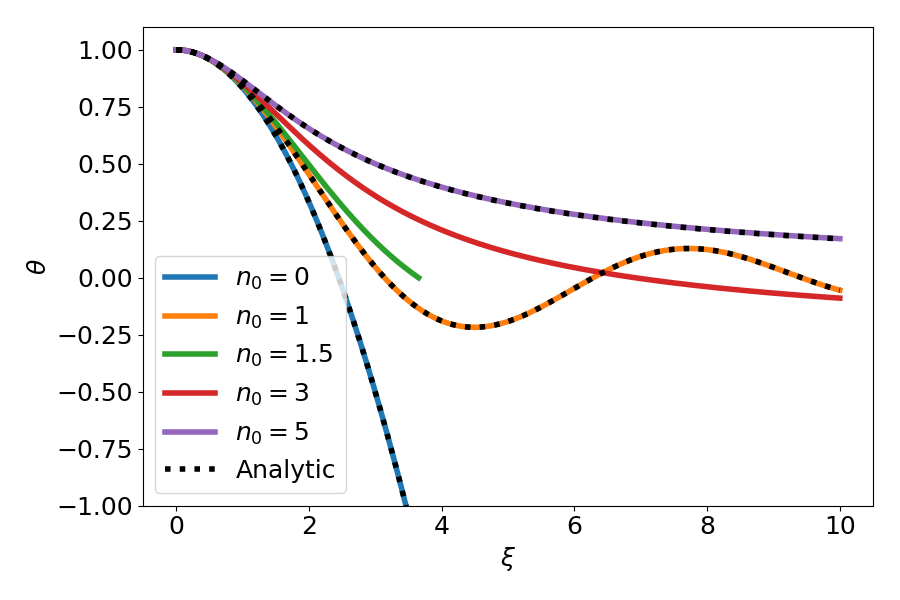
\includegraphics[width=.9\linewidth]{../plots/problem4.png}
\caption{\label{fig:problem4}The numerical solutions for part (b). Negative solutions are unphysical.}
\end{figure}
\end{document}
